\subsection{Analysis}\label{sec:analysis}

%Given the size of the groups, all results were statistically significant.

Aside from SF in the SFD measure, and Adjusted nDCG, BC was the best performing method.

\begin{figure}[H]
	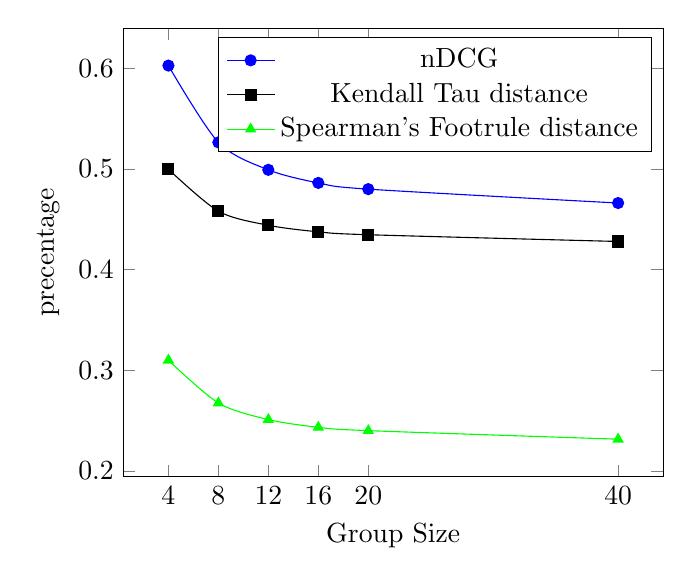
\begin{tikzpicture}
	\begin{axis}[
	xlabel=Group Size,
	ylabel=precentage,
	xtick = {4,8,12,16,20,40}]
	\addplot[smooth,mark=*,blue] plot coordinates {
		(4,0.6028)
		(8,0.5265)
		(12,0.4992)
		(16,0.4862)
		(20,0.48)
		(40,0.4662)
	};
	\addlegendentry{nDCG}
	
	\addplot[smooth,color=black,mark=square*] plot coordinates {
		(4,0.4998)
		(8,0.4581)
		(12,0.4441)
		(16,0.4376)
		(20,0.4347)
		(40,0.428)
	};
	\addlegendentry{Kendall Tau distance}
	
	\addplot[smooth,color=green,mark=triangle*] plot coordinates {
		(4,0.31)
		(8,0.2675)
		(12,0.251)
		(16,0.2433)
		(20,0.24)
		(40,0.2315)
	};
	\addlegendentry{Spearman's Footrule distance}
	
	\end{axis}
	\end{tikzpicture}
	\caption{Results for Borda Count}\label{fig:ndcganalysis}
\end{figure}

